\documentclass[10pt]{article}
\usepackage[margin=0.92in]{geometry}
\usepackage{amsmath,amssymb}
\usepackage{booktabs}
\usepackage{graphicx}
\usepackage{cite}
\usepackage{tikz}
\usetikzlibrary{positioning,arrows.meta}
\usepackage{setspace}
\setstretch{1.12}

\title{Perspective Lattice Completion for Side-View Counting\\ of Stacked Beer Crates}
\author{Computer Science\\ System Design and Optimization}
\date{}

\begin{document}
\maketitle

\begin{abstract}
Beer crates on a forklift are a regular lattice seen from the side. A mask count of that face misses the ranks behind it and also misses shadowed or clipped cells. This paper estimates the count by snapping rectified mask centers to the known crate pitch, filling a single empty cell that has two orthogonal neighbors, and multiplying by a depth reading. On a Monte Carlo model of detection, the lattice counter has mean absolute error $3.01$ crates against $4.87$ for masks times depth, $7.26$ for an area ratio, and $3.31$ for a span fill of the bounding rectangle. Unioning five frames at a vote of one raises the error to $5.80$ with a positive bias of $5.33$. The recommended counter uses one frame.
\end{abstract}

\noindent\textbf{Keywords---}object counting, instance segmentation, lattice, warehouse inventory.

\section{Introduction}
The image at a brewery gate shows the front face of a stack. The count the warehouse needs includes the crates behind that face. If the pallet is three deep, a perfect segmentation of the visible face is wrong by a factor of three. No gain in mask average precision repairs a factor of three. Depth is a small integer, one to three in the loads considered here, and it is treated as a reading with a known error rate rather than as something the side image is asked to invent.

The front face itself is not a crowd. Returnable crates of one family have a nominal face of $0.40\,\mathrm{m}$ by $0.28\,\mathrm{m}$. They are placed on a palletizer grid. Centers that survive detection fall nearer to their own cell than to a neighbor, once the face has been rectified. That regularity is the information an area ratio does not use and a density map cannot store. Perspective lattice completion (PLC) turns it into an integer: occupied cells on the rectified face, times the depth reading.

The estimate uses a generator of stacks and of missed detections. It is not a count from a filmed passage. The comparison is still informative, because every counter sees the same centers and the same depth reading.

\section{Related work}
Learned counters that integrate a density were built for crowds and for dotted annotations~\cite{lempitsky2010,li2018}. The integral does not remember color, and it does not add a hidden rank. Detection counting preserves identity and is biased low by every miss. An area-ratio inventory divides each visible mask by a nominal full area and sums the fractions~\cite{hu2025}. On tobacco cargo with Mask2Former that ratio is a reported inventory accuracy of $93.90\%$. The ratio is the right tool when the goods have no pitch. When the pitch is known, a fraction below one is a biased estimator of a cell that is either present or absent.

Counting stacked identical objects from several views can be posed as a volume times an occupancy ratio~\cite{dumery2024}. That decomposition fits a jumble in a bin. It is a poor fit to an integer depth of identical crates and a single side view lasting a second or two. Rotated lightweight detectors address yaw and occlusion of logistics boxes~\cite{wang2025} and still return boxes, not a depth-multiplied lattice. A carton dataset shows that repeated texture glues neighboring boxes~\cite{yang2022}. PLC does not repaint that seam. If two crates arrive as one center, they snap to one cell. The lattice repairs holes, not systematic merges.

\section{Method}
\subsection{The count}
Index front cells by row $r$, upward from the pallet, and column $c$. Let $O_{r,c}\in\{0,1\}$ and let $d\in\{1,2,3\}$ be the depth in crates. Under the regularity that a missing front cell means the ranks behind it are missing as well,
\begin{equation}
N=d\sum_{r,c}O_{r,c}.
\label{eq:truth}
\end{equation}
The side image does not observe $d$ or every $O_{r,c}$. PLC estimates the occupied set $\mathcal{F}$ and sets $\hat N=\hat d\,|\mathcal{F}|$.

\subsection{Rectification, origin, and snap}
A homography $H$, fit once at installation from a planar target~\cite{zhang2000,hartley2004}, sends a mask center to metres $(x,y)$ on the front plane. The pitch $(w,h)=(0.40,0.28)$ is known and the origin is not, because the truck does not stop on a mark. The origin is the median residual of the centers after each has been snapped to a lattice that was temporarily given origin zero:
\begin{equation}
\begin{aligned}
o_x&=\mathrm{median}_i\Big(x_i-\big(\mathrm{round}(x_i/w-\tfrac12)+\tfrac12\big)w\Big),
\end{aligned}
\label{eq:origin}
\end{equation}
and likewise for $o_y$. The median resists false centers up to half the set. The cell is then
\begin{equation}
c=\mathrm{round}\big((x-o_x)/w-\tfrac12\big),
\label{eq:snap}
\end{equation}
and likewise for the row. If the origin is exact and the noise is smaller than half a cell on each axis, the snap returns the true cell. Half a cell is $20\,\mathrm{cm}$ across. The noise used later has standard deviation $3.5\,\mathrm{cm}$ across and $2.8\,\mathrm{cm}$ vertically, so rounding is rarely the error. Missed detections are the error.

\subsection{One pass of completion}
Let $\mathcal{D}$ be the cells that received a center, and let $\mathcal{F}$ start as $\mathcal{D}$. Inside the bounding rectangle, an empty cell is added if at least two of its four orthogonal neighbors are already in $\mathcal{F}$. The pass is left to right, bottom to top, and the update is immediate. One neighbor is the outside of a solid stack and must not grow a rind. Two neighbors is the corner of a hole. The same test fills a step in the true outline: a top row that really contains only the right-hand crate presents the empty cell beside it with a lower neighbor and a right neighbor.

\begin{figure}[t]
\centering
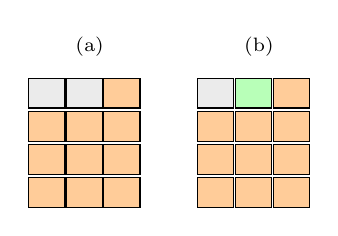
\begin{tikzpicture}[
  font=\scriptsize,
  c/.style={draw, minimum width=4.6mm, minimum height=3.8mm, inner sep=0pt},
  on/.style={c, fill=orange!40},
  off/.style={c, fill=black!8},
  add/.style={c, fill=green!28}
]
\node at (0.55,1.85) {(a)};
\foreach \r in {0,1,2} {\foreach \col in {0,1,2} {\node[on] at (\col*0.48,\r*0.42) {};}}
\node[off] at (0,1.26) {};
\node[off] at (0.48,1.26) {};
\node[on] at (0.96,1.26) {};
\begin{scope}[shift={(2.15,0)}]
\node at (0.55,1.85) {(b)};
\foreach \r in {0,1,2} {\foreach \col in {0,1,2} {\node[on] at (\col*0.48,\r*0.42) {};}}
\node[off] at (0,1.26) {};
\node[add] at (0.48,1.26) {};
\node[on] at (0.96,1.26) {};
\end{scope}
\end{tikzpicture}
\caption{A stepped top row. (a) Truth: one crate on the top right. (b) After one left-to-right pass the middle top cell, which has two orthogonal neighbors, is filled. The corner is visited first and stays empty.}
\label{fig:step}
\end{figure}

Depth is not inferred from the masks. The reading $\hat d$ equals $d$ with probability $0.90$ and otherwise moves by one, clipped to $\{1,2,3\}$. A wrong reading costs about $|\mathcal{F}|$ crates. No gap rule repairs it, so the reading is shown beside the total.

A union of frames with vote threshold one is the obvious robust variant and the one the estimate rejects. False cells that never co-occur in a single frame become mutual neighbors in the union, and immediate update then adds more. The bound that one false center adds at most one cell is true of one frame and false of the union.

\subsection{Baselines that share the reading}
The mask tally is the number of centers and ignores depth. Mask times depth multiplies that number by $\hat d$. The area ratio sums a visible fraction of mean $0.86$ for each detection, rounds, and multiplies by $\hat d$. The span estimates rows and columns from the robust extent of the point cloud divided by the pitch, fills that rectangle solid, and multiplies by $\hat d$. PLC is the span's use of pitch, plus a refusal to fill unsupported cells, plus a willingness to fill one supported hole.

\section{Estimate}
Each trial draws two to six rows, two to four columns, and depth one to three. Cells are occupied with probability $0.93$. A blur variable lowers detection probability by up to $0.18$. At zero blur the bottom row is kept with probability $0.70$, the top with $0.84$, and a middle row with $0.96$. A detected center is the cell center plus the Gaussian noise above. False centers arrive as a Poisson count of mean $0.35$. Five frames are drawn. Four thousand trials are run. The mean truth is $22.62$ crates.

\begin{table}[t]
\caption{Counting error on $4000$ stacks. Bias is the mean of $\hat N-N$.}
\label{tab:count}
\centering
\footnotesize
\setlength{\tabcolsep}{2.6pt}
\begin{tabular}{@{}lrrrr@{}}
\toprule
Counter & MAE & Bias & Exact & P90 $|e|$ \\
\midrule
Mask, no depth & $13.55$ & $-13.53$ & $0.044$ & $31$ \\
Mask $\times$ depth & $4.87$ & $-4.33$ & $0.126$ & $12$ \\
Area ratio & $7.26$ & $-7.08$ & $0.030$ & $15$ \\
Span lattice & $3.31$ & $+1.60$ & $0.332$ & $9$ \\
PLC, one frame & $3.01$ & $+0.83$ & $0.337$ & $8$ \\
PLC, five-frame union & $5.80$ & $+5.33$ & $0.221$ & $15$ \\
\bottomrule
\end{tabular}
\end{table}

Table~\ref{tab:count} separates three effects. Ignoring depth is an almost pure under-count: mean absolute error $13.55$ and bias $-13.53$. Multiplying the same masks by the reading cuts the absolute error to $4.87$. That is the largest single reduction. The area ratio is worse than those masks, because a fraction centered at $0.86$ short-changes a stack that was already slightly short. This does not refute an area-ratio result on irregular cargo~\cite{hu2025}. It says a fraction below one is the wrong summary of a missed crate of known size.

Given depth, the span reaches absolute error $3.31$ and bias $+1.60$. PLC on one frame reaches $3.01$ and $+0.83$, and is exact on $0.337$ of trials. The absolute gap is three tenths of a crate on a load of about twenty-three. The bias gap is the signature of the neighbor test: both methods over-fill, and the test over-fills less than a solid rectangle. The five-frame union is a nearly pure over-count, bias $+5.33$ against absolute error $5.80$. Five frames are worse than one. By true depth, PLC on one frame stays ahead of the span: absolute errors $1.72$, $3.27$, and $4.03$ at depths one, two, and three, against $1.91$, $3.59$, and $4.40$.

One drawn stack makes the positive bias countable. The front occupancy is three full rows of three and a top row with only the right-hand crate, ten cells, depth two, truth $20$. The first frame has nine detections. The rule restores the miss and also fills the middle of the top step, eleven cells, booked total $22$. The span fills both empty top cells and books $24$. The five-frame union books $28$. The hand rule and the instrument agree with each other and not with the truth.

A wrong depth reading contributes on the order of one crate of absolute error when the front has about ten cells and the error rate is ten percent. That term is shared by every counter that multiplies by $\hat d$. Halving the rate is worth about as much as the entire gap between the span and PLC. The design priority is a depth value from the pallet record, and vision effort spent on the front face.

\section{What is displayed}
The booked record shows the total, the completed-cell count $|\mathcal{F}\setminus\mathcal{D}|$, the median origin residual, and whether $\hat d$ was a default. An exact total with a positive completed-cell count can be a cancellation: one unrestored miss and one phantom. The exact-match rate of $0.337$ is not the fraction of passages that were correct for the right reason. The bias under one crate says phantoms slightly outweigh remaining misses. A passage is refused when the buffer is empty or the origin residual exceeds half a cell. A zero count is reserved for an empty pallet.

\section{What this estimate does not say}
The detection probability already folds shadow, blur, and suppression into one number per row. A real threshold on non-maximum suppression would have to be tuned against labeled frames before anyone treated Table~\ref{tab:count} as a prediction of that threshold. Merged seams are the other gap. If two crates arrive as one center, they occupy one cell, and the fill rule does not invent the missing neighbor unless some other detection supports it. The vertical-feature gate in the baseline segmenter is the intended defense against that merge. This paper does not estimate the gate.

The visit order is part of the method that was measured. A right-to-left pass on the stepped stack would fill the corner as well as the middle cell, and PLC would then agree with the span at $24$ on the worked example. Changing the order is a different counter and needs its own row. The row in the table is left to right, immediate update, threshold two.

\section{Conclusion}
Side-view crate counting is a lattice times an integer depth, not a density and not a sum of partial areas. Snapping centers to the known pitch and filling only a doubly supported hole is a small improvement on filling the bounding span and a large improvement on counting masks. The improvement does not justify fusing every frame of the passage at a vote of one: that union invents cells. The counter to run is PLC on the single sharpest frame, with the depth reading shown beside the total, until a filmed gate says otherwise.

\begin{thebibliography}{99}
\bibitem{lempitsky2010} V.~Lempitsky and A.~Zisserman, ``Learning to count objects in images,'' in \emph{NeurIPS}, 2010.
\bibitem{li2018} Y.~Li, X.~Zhang, and D.~Chen, ``CSRNet: Dilated convolutional neural networks for understanding the highly congested scenes,'' in \emph{CVPR}, 2018, pp.~1091--1100.
\bibitem{hu2025} X.-M.~Hu, B.-H.~Wang, and Z.~Yang, ``Area ratio-based box counting algorithm for intelligent inventory in stacked goods environments,'' in \emph{MiTA}, 2025, pp.~1--9.
\bibitem{dumery2024} C.~Dumery, N.~Ett\'e, A.~Fan, R.~Li, J.~Xu, H.~Le, and P.~Fua, ``Counting stacked objects,'' arXiv:2411.19149, 2024.
\bibitem{wang2025} G.~Wang \emph{et al.}, ``REW-YOLO: A lightweight box detection method for logistics,'' \emph{Modelling}, vol.~6, no.~3, p.~76, 2025.
\bibitem{yang2022} J.~Yang \emph{et al.}, ``SCD: A stacked carton dataset for detection and segmentation,'' \emph{Sensors}, vol.~22, no.~10, p.~3617, 2022.
\bibitem{zhang2000} Z.~Zhang, ``A flexible new technique for camera calibration,'' \emph{IEEE Trans. Pattern Anal. Mach. Intell.}, vol.~22, no.~11, pp.~1330--1334, 2000.
\bibitem{hartley2004} R.~Hartley and A.~Zisserman, \emph{Multiple View Geometry in Computer Vision}, 2nd~ed. Cambridge Univ. Press, 2004.
\bibitem{bolya2019} D.~Bolya, C.~Zhou, F.~Xiao, and Y.~J.~Lee, ``YOLACT: Real-time instance segmentation,'' in \emph{ICCV}, 2019, pp.~9157--9166.
\bibitem{cheng2022} B.~Cheng, I.~Misra, A.~G.~Schwing, A.~Kirillov, and R.~Girdhar, ``Masked-attention mask transformer for universal image segmentation,'' in \emph{CVPR}, 2022, pp.~1290--1299.
\end{thebibliography}

\end{document}
